\chapter{Partial derivative} \label{ch6ch}

Partial derivative studies the effect of a small deviation of one particular independent variable on the multivariable function. It is similar with the normal derivative in many ways, but also has its unique characteristics.

In Section \ref{ch6sec:motivatingexp}, a motivating example is given to illustrate the motivation of introducing partial derivative. In Section \ref{ch6sec:partialtotalderivative}, the definition of partial derivative is given. In Sections \ref{ch6sec:gradient} and \ref{ch6sec:jacobianmatrix}, two very important and commonly used tool derived from partial derivative, namely gradient and Jacobian matrix, are introduced respectively.

\section{A Motivating Example} \label{ch6sec:motivatingexp}

Consider the following motivating example where $y=f(x_1, x_2)$ is a multivariable function with $2$ inputs.

\begin{shortbox}
\Boxhead{A Motivating Example}

Consider
\begin{eqnarray}
    y &=& 2x_1^2 + x_2^2 + 2x_1x_2. \label{ch6eq:motivatingexample}
\end{eqnarray}

Q1: Let $x_2 = 1$ be a constant. Derive $y$ as a function of $x_1$, and calculate its derivative with respect to $x_1$. Similarly, let $x_1 = 1$ be a constant and derive $y$ as a function of $x_2$, and calculate its derivative with respect to $x_2$.

Q2: At $(x_1, x_2) = (1, 1)$, consider small vibrations $\Delta x_1$ and $\Delta x_2$. Approximate $\Delta y$ as a function of $\Delta x_1$ and $\Delta x_2$ using differentiation.

Q3: Find such $x_1$ and $x_2$ that $y$ is minimized.

\end{shortbox}

Equation \eqref{ch6eq:motivatingexample} can be plot in 3-D as Fig. \ref{ch6fig_motivatingexp}.
\begin{figure}
	\centering
	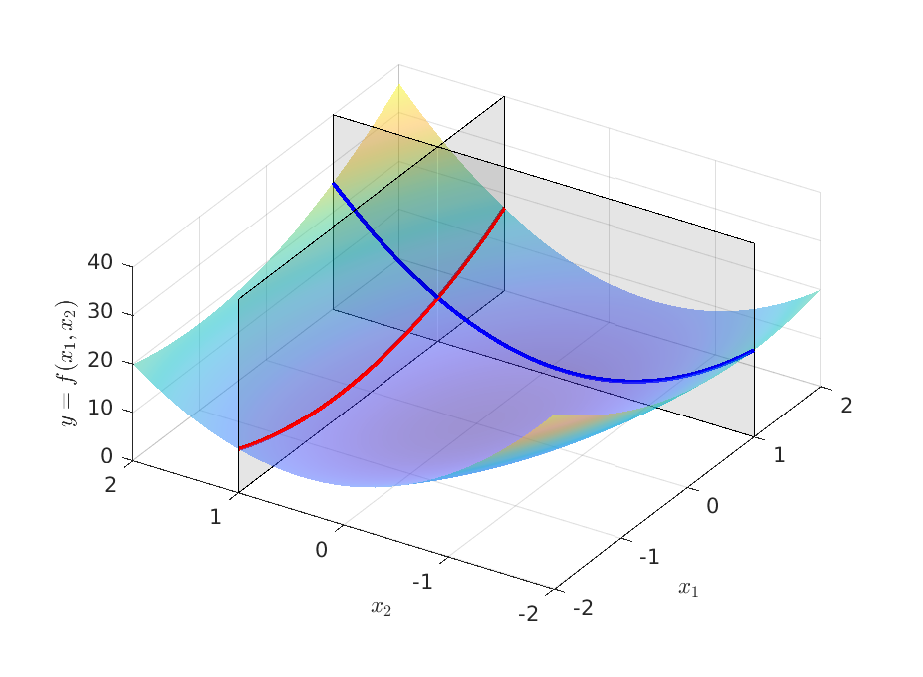
\includegraphics[width=250pt]{chapters/chapter6/figures/fig_motivatingexp.eps}
	\caption{Plot of function $y=f(x_1, x_2)$ in 3-D.} \label{ch6fig_motivatingexp}
\end{figure}

Let $x_2=1$ be constant. Equation \eqref{ch6eq:motivatingexample} becomes
\begin{eqnarray}
	y = f(x_1, 1) = 2x_1^2 + 2x_1 + 1, \nonumber
\end{eqnarray}
which is given by the intersection of  curved surface (equation \eqref{ch6eq:motivatingexample}) and the vertical flat ($x_2=1$) given by the red solid line in Fig. \ref{ch6fig_motivatingexp}. Its derivative with respect to $x_1$ can be easily obtained as
\begin{eqnarray}
	\dfrac{d}{dx_1}f(x_1,1) &=& 4x_1 + 2. \label{ch6eq:motivatingexpdx1}
\end{eqnarray}

Similarly, at $x_1 = 1$, \eqref{ch6eq:motivatingexample} becomes
\begin{eqnarray}
	y = f(1, x_2) = x_2^2 + 2x_2 + 2, \nonumber
\end{eqnarray}
which is given by the blue solid line in Fig. \ref{ch6fig_motivatingexp}. Its derivative with respect to $x_2$ is
\begin{eqnarray}
	\dfrac{d}{dx_2}f(1,x_2) &=& 2x_2 + 2. \label{ch6eq:motivatingexpdx2}
\end{eqnarray}

Consider small vibrations $\Delta x_1$ and $\Delta x_2$. Firstly, let $x_2$ remain constant and only apply $\Delta x_1$ on $y = f(1,1)$. In this case,
\begin{eqnarray}
	\Delta y = f(1+\Delta x_1, 1) - f(1, 1) \approx \dfrac{d}{dx_1}f(x_1,1) \Delta x_1, \label{ch6eq:partialdifx1}
\end{eqnarray}
where $\dfrac{d}{dx_1}f(x_1,1)$ is given in \eqref{ch6eq:motivatingexpdx1}.

On top of \eqref{ch6eq:partialdifx1}, consider vibration $\Delta x_2$. The derivative of function $f(1+\Delta x_1, x_2)$ with respect to $x_2$ depends on $\Delta x_1$ and it is generally unknown without specifying $\Delta x_1$. However, since \eqref{ch6eq:motivatingexample} is continuous and ``smooth'' (Notice that ``smooth'' has specific definition in mathematics. Here, just take its literal meaning: it is perfectly polished without any edges or spikes.), we can intuitively understand that when $\Delta x_1$ is small, $\frac{d}{dx_2}f(1+\Delta x_1, x_2) \approx \frac{d}{dx_2}f(1, x_2)$, and $\frac{d}{dx_2}f(1+\Delta x_1, x_2) \rightarrow \frac{d}{dx_2}f(1, x_2)$ as $\Delta x_1 \rightarrow 0$. Thus, we have
\begin{eqnarray}
	\Delta y &=& \left(f(1+\Delta x_1, 1 + \Delta x_2) -  f(1+\Delta x_1, 1)\right) + \left(f(1+\Delta x_1, 1) - f(1, 1)\right) \nonumber \\
	&\approx& \dfrac{d}{dx_2}f(1,x_2) \Delta x_2 + \dfrac{d}{dx_1}f(x_1,1) \Delta x_1. \label{ch6eq:motivatingresult1}
\end{eqnarray}

In \eqref{ch6eq:motivatingresult1}, consider $\Delta x_1 \rightarrow 0$ and $\Delta x_2 \rightarrow 0$. Denote such $\Delta x_1$ and $\Delta x_2$ as $dx_1$ and $dx_2$ respectively, and the associated $\Delta y$ as $dy$. Here ``$d(\cdot)$'' represents the \textit{infinitesimal change}. Equation \eqref{ch6eq:motivatingresult1} then becomes
\begin{eqnarray}
	d y &=& \dfrac{d}{dx_2}f(1,x_2) d x_2 + \dfrac{d}{dx_1}f(x_1,1) d x_1. \label{ch6eq:motivatingresult2}
\end{eqnarray}

Equation \eqref{ch6eq:motivatingresult2} can be extended to more general cases where $(x_1, x_2) = (1, 1)$ is not specified. The terms $\dfrac{d}{dx_1}f(x_1,1)$ and $\dfrac{d}{dx_2}f(1,x_2)$ needs to be changed accordingly. For example, $\dfrac{d}{dx_1}f(x_1,1)$ given by \eqref{ch6eq:motivatingexpdx1} shall be changed to
\begin{eqnarray}
	\left.\dfrac{d}{dx_1}f(x_1,x_2)\right|_{x_2 \textup{~is constant}} &=& 4x_1 + 2x_2 \nonumber
\end{eqnarray} 
with $x_2$ being any arbitrary constant. 

The denotation $\left.\dfrac{d}{dx_1}f(x_1,x_2)\right|_{x_2 \textup{~is constant}}$ can sometimes become ambiguous if not handled carefully. One of the reasons could be that ``$d(\cdot)$'' is used as infinitesimal change as shown before. In this case both $dx_1$ and $dx_2$ contribute to $df(x_1,x_2)$, but we would want $\dfrac{d}{dx_1}f(x_1,x_2)$ here to reflect the deviation of $f(x_1,x_2)$ caused by $dx_1$ only, and it is not convenient to list down all the other variables and put ``is/are constant'' everywhere in the equation. Therefore, instead of saying $\left.\dfrac{d}{dx_1}f(x_1,x_2)\right|_{x_2 \textup{~is constant}}$, we denote 
\begin{eqnarray}
	\dfrac{\partial}{\partial x_1} f(x_1, x_2) &=& 4x_1 + 2x_2. \nonumber
\end{eqnarray}
The operator $\dfrac{\partial}{\partial x}$ is called \textit{partial derivative} (with respect to $x$), often followed by a multivariable function $f(x,y)$ where $x$ is one of its inputs. It is similar to the derivative, but emphasizing that the interested function is multivariable, and the derivative of this function with respect to ONLY ONE variable is being studied (and the rest variables assumed constant). Since $\partial f(x)$ is rarely or never used as the infinitesimal of $f(x)$, it will hopefully be less ambiguous.

The formal definition of $\partial x$ is given in next Section \ref{ch6sec:partialtotalderivative}.

Equation \eqref{ch6eq:motivatingresult2} for general $(x_1,x_2)$, therefore, becomes
\begin{eqnarray}
	d y &=& \dfrac{\partial}{\partial x_2}f(x_1,x_2) d x_2 + \dfrac{\partial}{\partial x_1}f(x_1,x_2) d x_1. \label{ch6eq:motivatingtotaldiff}
\end{eqnarray}

The minimum $y=f(x_1,x_2)$ and its associated $x_1$ and $x_2$ can be found by rewriting \eqref{ch6eq:motivatingexample} as
\begin{eqnarray}
	y &=& x_1^2 + \left(x_1 + x_2\right)^2. \nonumber
\end{eqnarray}
Therefore, the minimum $y$ is $y=0$, at $x_1 = 0$ and $x_1 + x_2 = 0$, i.e., $x_1 = x_2 = 0$.

This can also be solved using \eqref{ch6eq:motivatingtotaldiff}. At the minimum point of $y$, $\dfrac{\partial}{\partial x_2}f(x_1,x_2)$ and $\dfrac{\partial}{\partial x_1}f(x_1,x_2)$ must both zero. Otherwise, it is always possible to add/subtract a small $\Delta x_1$ or $\Delta x_2$ to further decrease $y$. Thus, from \eqref{ch6eq:motivatingexample}
\begin{eqnarray}
	\dfrac{\partial}{\partial x_1}f(x_1,x_2) &=& 4x_1 + 2x_2 = 0 \nonumber \\
	\dfrac{\partial}{\partial x_2}f(x_1,x_2) &=& 2x_1 + 2x_1 = 0
\end{eqnarray}
which yields $x_1=x_2=0$.

\section{Partial and Total Derivative} \label{ch6sec:partialtotalderivative}

\section{Gradient} \label{ch6sec:gradient}

\section{Jacobian Matrix} \label{ch6sec:jacobianmatrix}
